\chapter{Fundamentação Teórica}
% Reinicia numeração de tabelas para este capítulo
\setcounter{table}{0}

Este capítulo reúne a fundamentação teórica necessária, cobrindo conceitos de computação em nuvem, virtualização, nuvens privadas, arquitetura do OpenStack e princípios de elasticidade e provisionamento dinâmico de recursos.

\section{Computação em Nuvem (\textit{Cloud Computing})}
\label{sec:cloud-computing}

\subsection{Definição e Paradigma}

A computação em nuvem (\textit{cloud computing}) é definida na publicação especial 800-145 pelo \textit{National Institute of Standards and Technology}(NIST), como um modelo que permite acesso a um conjunto compartilhado de recursos computacionais configuráveis, como redes, servidores, armazenamento, aplicações e serviços,  sob demanda e via rede. Esses recursos podem ser rapidamente provisionados e liberados com mínimo esforço de gerenciamento ou interação com o provedor de serviços \cite{mell2011}. Essa definição enfatiza características essenciais da computação em nuvem, dentre as quais destacam-se:

\begin{description}
    \item[Autoatendimento sob demanda (\textit{On-demand self-service})]: o usuário pode provisionar recursos computacionais, como tempo de servidor e armazenamento em rede, conforme a necessidade, automaticamente e sem necessidade de interação humana com cada provedor de serviço \cite{mell2011};
    \item[Acesso amplo à rede (\textit{Broad network access})]: os serviços da nuvem podem ser acessados pela grande maioria de aparelhos que possuem acesso à internet, com interfaces padronizadas que facilitam a experiência dos usuários que já estão acostumados com algum serviço na nuvem \cite{mell2011};
    \item[Agrupamento de recursos (\textit{Resource pooling})]: CPU, RAM, armazenamento e largura de banda de rede, são agrupados pelo provedor para atender múltiplos inquilinos usando um modelo de multilocação (\textit{multi-tenant}), com diferentes recursos sendo distribuídos dinamicamente e redistribuídos conforme a demanda do inquilino \cite{mell2011};
    \item[Elasticidade rápida (\textit{Rapid elasticity})]: os recursos podem ser provisionados e liberados elasticamente, em alguns casos automaticamente, para escalar rapidamente conforme a demanda. Para o usuário, as capacidades disponíveis para provisionamento parecem ser ilimitadas, a depender da quantidade de hardware que o provedor possui,  e podem ser utilizadas em qualquer quantidade, a qualquer momento \cite{mell2011};
    \item[Serviço mensurado (\textit{Measured service})]: os sistemas de nuvem controlam e otimizam automaticamente o uso de recursos utilizando recursos de medição. Devido a isso, o uso dos recursos pode ser monitorado, controlado e reportado, proporcionando transparência tanto para o provedor quanto para o consumidor do serviço utilizado \cite{mell2011}.
\end{description}

\subsection{Modelos de Serviço}

Além dessas características essenciais, o NIST também classifica os serviços oferecidos por provedores de nuvem em três modelos de serviço:

\begin{description}
    \item[Software como Serviço (SaaS)]: oferece aplicações completas hospedadas na nuvem e acessadas pela internet. O usuário não gerencia a infraestrutura subjacente \cite{mell2011};
    \item[Plataforma como Serviço (PaaS)]: provê um ambiente na nuvem para que o usuário implante aplicações próprias, sem administrar servidores, rede ou sistemas operacionais \cite{mell2011};
    \item[Infraestrutura como Serviço (IaaS)]: disponibiliza recursos fundamentais, como CPU, armazenamento e rede, permitindo ao usuário instalar sistemas operacionais e aplicações com controle limitado de rede \cite{mell2011}.
\end{description}

\begin{figure}[htb]
\centering
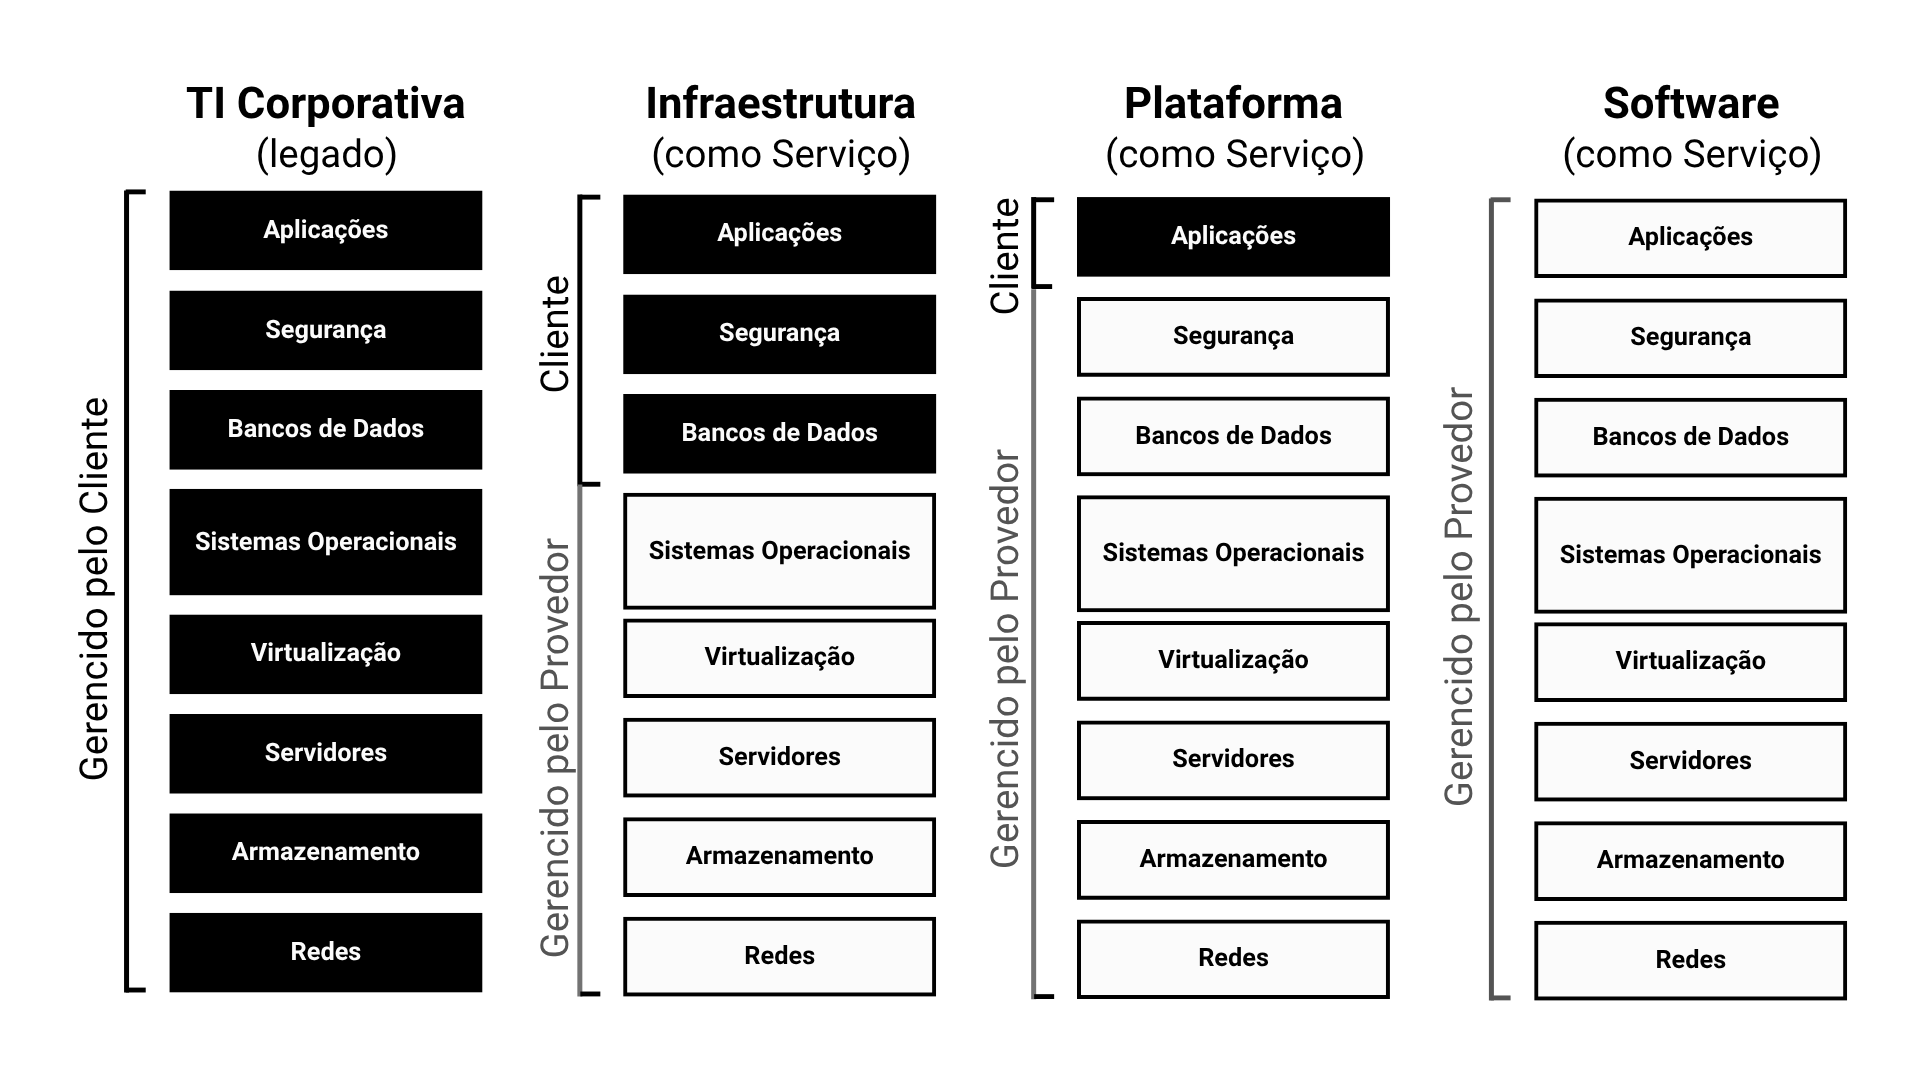
\includegraphics[width=0.8\textwidth]{figuras/Figura 1 - Comparação entre os modelos de serviço.png}
\caption{Comparação entre os modelos de serviço IaaS, PaaS e SaaS}
    \fonte{Adaptado de Rizvi et al. (2024).}
\label{fig:modelos-servico}
\end{figure}

Para facilitar o entendimento desses serviços, a Figura 1 compara os modelos de serviço da nuvem. Em sistemas de SaaS, o software é hospedado na nuvem e acessível ao usuário pela internet. O usuário não possui nenhum controle sobre a aplicação, nem sobre a infraestrutura. Grande parte dos serviços oferecidos à usuários da internet utilizam esse modelo \cite{rizvi2024}. Dentre eles, pode-se listar, as redes sociais, como o \textit{Instagram}, \textit{TikTok} e \textit{Whatsapp}, e serviços de transmissão contínua de conteúdo multimídia (\textit{streaming}), como o \textit{Youtube}, \textit{Netflix} e \textit{Spotify}. O modelo PaaS, em contrapartida, fornece um ambiente de desenvolvimento e implantação pré-construído na nuvem, onde o usuário tem controle sobre a aplicação, incluindo códigos e bancos de dados. Nesse modelo encontram-se os serviços de desenvolvimento e hospedagem de software, como \textit{Microsoft Azure}, \textit{Google App Engine} e \textit{Heroku} (Rizvi et al., 2024). Já no IaaS, o usuário pode solicitar uma quantidade de recursos, e tem controle sobre o sistema operacional (SO). Nesse modelo estão as máquinas virtuais e serviços de armazenamento, como  \textit{Amazon Web Services (AWS) EC2 e S3},  \textit{Microsoft Azure Virtual Machines} e  \textit{Google Compute Engine}  (Rizvi et al., 2024)

\subsection{Modelos de Implantação}

A implantação de sistemas de computação em nuvem pode ser realizada por meio de diferentes modelos, cada qual com características que determinam sua adequação a contextos específicos. Os modelos mais conhecidos são a nuvem pública, privada, comunitária e híbrida, os quais se diferenciam pelo nível de controle, segurança, escalabilidade e custo de implantação \cite{mell2011}.

\begin{description}
    \item[Nuvem Pública] - As nuvens públicas são gerenciadas por provedores terceirizados que disponibilizam recursos computacionais por meio da internet \cite{carroll2011}. Esses provedores costumam oferecer capacidades elevadas de escalabilidade e custos iniciais mais acessíveis, o que os torna atrativos para diferentes perfis de organizações \cite{amajuoyi2024}. Além disso, esse modelo de nuvem pode ser particularmente vantajoso para instituições que não contam com equipes internas especializadas no assunto ou que optam por não direcionar recursos à aquisição e manutenção de infraestrutura física própria. Em função desses benefícios, a adoção da nuvem pública tem apresentado um crescimento contínuo nos últimos anos \cite{amajuoyi2024}. Entretanto, as nuvens privadas podem apresentar desafios relevantes em termos de segurança e controle sobre a infraestrutura física. A nuvem pública é aberta a todos e sem garantia de alto nível de segurança, podendo trazer riscos à confidencialidade dos dados, à proteção de informações estratégicas e à perda ou roubo de dados, sendo uma opção mais adequada para empresas com "baixas preocupações de segurança" \cite{sathya2023}.
    \item[Nuvem Privada] - A infraestrutura é fornecida para uso exclusivo de uma única organização. Essa infraestrutura pode ser de propriedade, de terceiros, ou uma combinação de ambos, e pode estar localizada dentro ou fora das instalações da organização \cite{mell2011}. Para organizações que desejam um grau elevado de controle, personalização e alto nível de segurança, as nuvens privadas podem se destacar como uma solução adequada \cite{swapna2023}. Isso possibilita o desenvolvimento de um ambiente seguro e adaptado às exigências particulares de instituições que necessitam resguardar pesquisas sigilosas e proteger a propriedade intelectual. Dessa forma, a nuvem privada se mostra a alternativa ideal para operações que demandam um rigoroso gerenciamento de dados e confidencialidade, assegurando a integridade de informações estratégicas e o cumprimento de normativas internas.
    \item[Nuvem Comunitária] - A infraestrutura é fornecida para uso exclusivo de uma comunidade específica de clientes, pertencentes a diferentes organizações que compartilham interesses comuns. A infraestrutura pode ser de propriedade, de terceiros, ou uma combinação desses, e pode estar localizada dentro ou fora das instalações das organizações envolvidas \cite{mell2011}.
    \item[Nuvem Híbrida] - Essa infraestrutura é uma composição de duas ou mais infraestruturas distintas (privada, comunitária ou pública)  \cite{mell2011}.
\end{description}

A implantação de sistemas de computação em nuvem pode ser realizada por meio de diferentes modelos, cada qual adequado a cenários específicos. Os modelos mais difundidos são as nuvens pública, privada, comunitária e híbrida, que se diferenciam em nível de controle, segurança, escalabilidade e custo de implantação \cite{mell2011}.

\section{Virtualização e Hipervisores}
A virtualização é uma técnica de grande importância na computação moderna, uma vez  abstrai o hardware de máquinas físicas, agrupando logicamente os recursos de servidores. Esses agrupamentos lógicos, também conhecido como \textit{pools}, permite a criação de máquinas virtuais (VMs) isoladas em um único sistema computacional físico \cite{carissimi2008}; \cite{kominos2017}. Cada VM funciona como um ambiente de execução completo e autônomo, com sistema operacional próprio, aplicações, configurações e  serviços de rede, como se fosse uma máquina física independente \cite{carissimi2008}. Esta capacidade de particionamento lógico de recursos de hardware é um dos fundamentos da computação em nuvem, viabilizando a elasticidade, a multilocação e a eficiência de custos \cite{chawla2025}.

\subsection{Tipos de Virtualização}
A implementação de máquinas virtuais de sistema pode ser realizada através de duas técnicas principais:

\begin{description}
    \item[Virtualização Total]: Também conhecida como \textit{Máquina Virtual de Hardware (HVM)}, esse tipo de virtualização provê uma réplica virtual completa do hardware subjacente. Isso permite rodar qualquer sistema operacional usando sua imagem de instalação padrão (ISO) sem alterar o kernel \cite{carissimi2008}. O desafio da virtualização total reside no tratamento de comandos que precisam de acesso direto ao hardware, as instruções privilegiadas. Em princípio, a camada de virtualização precisava interceptar e emular essas instruções em software, gerando uma sobrecarga (\textit{overhead}) de desempenho \cite{carissimi2008}. Contudo, a introdução de extensões de hardware pelos fabricantes de processadores, como o \textit{Intel VT-x} e o \textit{AMD-V}, revolucionou essa técnica \cite{carissimi2008}. Essas extensões permitem que o sistema operacional virtualizado execute instruções privilegiadas diretamente no processador de forma segura, eliminando a necessidade de emulação e tornando o desempenho da máquina virtual mais próximo ao do hardware nativo \cite{chawla2025}.
    \item[Paravirtualização]: Essa é a técnica em que o sistema operacional é modificado para melhor se adaptar a um ambiente virtual. O \textit{kernel} do sistema é alterado para incluir \textit{drivers} especiais que realizam chamadas diretas ao hipervisor (hypercalls), em vez de tentar executar instruções privilegiadas, \cite{carissimi2008}. A principal vantagem desta abordagem é o desempenho. Ao eliminar a necessidade de interceptar e emular instruções, a paravirtualização apresenta um \textit{overhead} menor e um desempenho superior em comparação à virtualização total sem assistência de hardware \cite{carissimi2008}.
\end{description}

Para facilitar o entendimento dos conceitos da Virtualização Total e Paravirtualização, a Tabela~\ref{tab:comparativo_virtualizacao} apresenta um comparativo entre esses dois tipos, destacando suas vantagens e desvantagens:

\begin{table}[htb]
    \centering

    \caption{Comparativo entre Virtualização Total e Paravirtualização}
    \label{tab:comparativo_virtualizacao}

    \begin{tabularx}{\textwidth}{ l >{\raggedright\arraybackslash}X >{\raggedright\arraybackslash}X }
        \toprule
        \textbf{Característica} & \textbf{Virtualização Total} & \textbf{Paravirtualização} \\
        \midrule
        Visão do \textit{Guest} & Hardware virtual idêntico ao físico. & API/hardware simplificado, exposto pelo hipervisor. \\
        \addlinespace
        Modificação do SO & Não é necessária. & Sim, o \textit{kernel} precisa de drivers e \textit{hypercalls} especiais. \\
        \addlinespace
        Instruções Privilegiadas & Interceptadas pelo hipervisor ou tratadas via hardware (\textit{Intel VT-x/AMD-V}). & O \textit{guest} realiza \textit{hypercalls} diretas ao hipervisor. \\
        \addlinespace
        Desempenho & Historicamente mais lento, mas hoje quase nativo graças à assistência de hardware. & Menor sobrecarga e desempenho superior, especialmente em I/O. \\
        \addlinespace
        Principal Vantagem & Compatibilidade universal com qualquer sistema operacional. & Velocidade e eficiência, sobretudo antes da popularização do \textit{Intel VT-x}. \\
        \addlinespace
        Principal Desvantagem & Maior sobrecarga sem assistência de hardware. & Requer suporte e modificação no sistema operacional convidado. \\
        \bottomrule
    \end{tabularx}

    \fonte{Elaborado pelo autor, com base em Carissimi (2008).}
\end{table}


\subsection{Definição e tipos de hipervisores}
O componente de software responsável por criar e gerenciar as máquinas virtuais é denominado hipervisor, ou Monitor de Máquina Virtual (VMM) \cite{chawla2025}; \cite{carissimi2008}. O hipervisor é a camada de software que fica entre o hardware e os sistemas operacionais, e é responsável por orquestrar o acesso aos recursos físicos e manter o isolamento entre as diferentes VMs \cite{chawla2025}; \cite{carissimi2008}. Os hipervisores são classificados em dois tipos principais, conforme ilustrado na Figura 2.

\begin{figure}[htb]
    \centering
    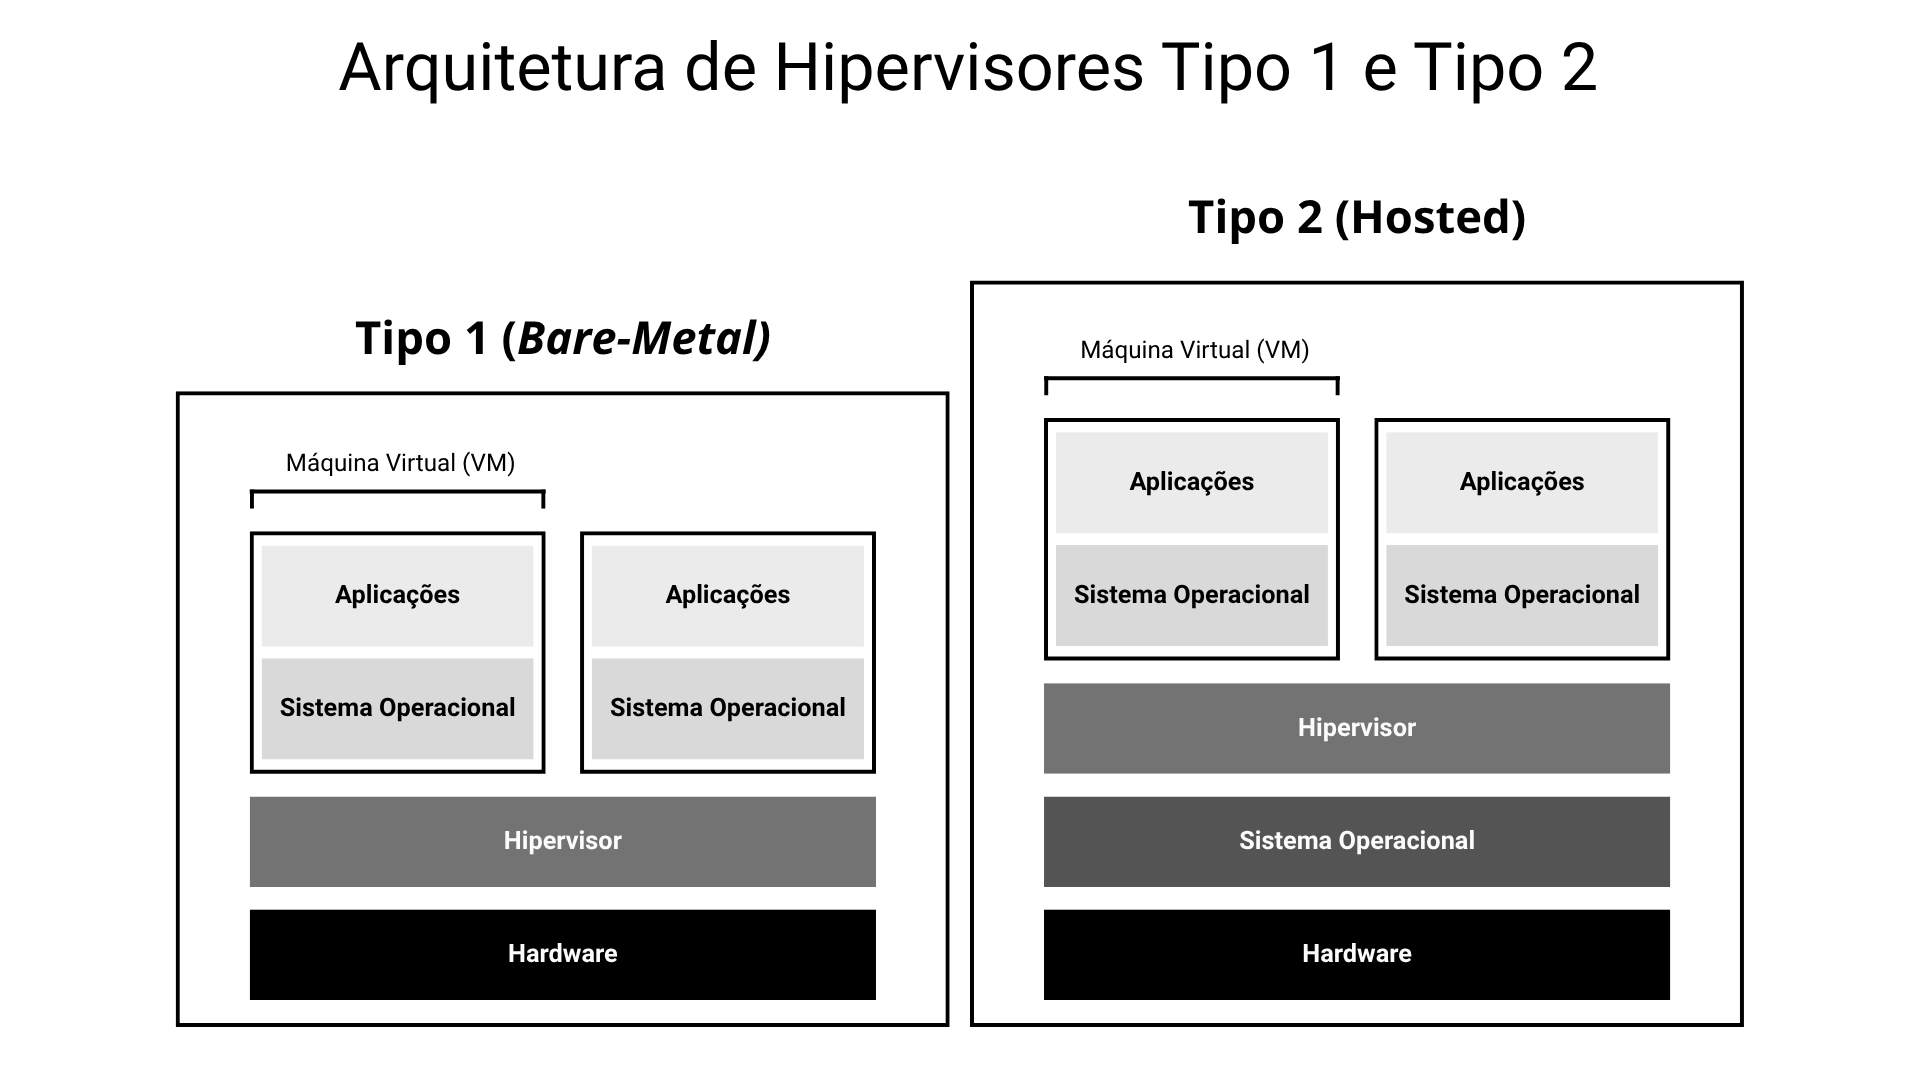
\includegraphics[width=0.8\textwidth]{figuras/Figura 2 - Arquitetura de Hipervisores.png}
    \caption{Arquiteturas de hipervisores do Tipo 1 (bare-metal) e Tipo 2 (hosted).}
        \fonte{Adaptado de Chawla et al. (2025).}
    \label{fig:arquitetura-hipervisores}
\end{figure}


\begin{description}
    \item[Tipo 1 (\textit{Bare-metal})]: Executa diretamente sobre o hardware do servidor, atuando como um sistema operacional leve e especializado para executar VMs \cite{chawla2025}. Exemplos notáveis incluem \textit{Xen}, \textit{VMware ESXi} e \textit{Microsoft Hyper-V} \cite{chawla2025}; \cite{carissimi2008}. Por ter acesso direto ao hardware, esta arquitetura geralmente oferece maior desempenho e segurança.
    \item[Tipo 2 (\textit{Hosted})]: Opera como uma aplicação de software sobre um sistema operacional convencional (hospedeiro), que gerencia o hardware \cite{chawla2025}. Exemplos incluem \textit{KVM}, \textit{Oracle VirtualBox} e \textit{VMware Player} \cite{chawla2025}; \cite{carissimi2008}. Esta abordagem é mais simples de instalar e gerenciar, mas pode introduzir uma sobrecarga de desempenho devido à camada extra do sistema operacional hospedeiro.
\end{description}

A Tabela~\ref{tab:comparativo_hipervisores} compara, de forma simplificada, as diferenças entre os hipervisores Tipo~1 e Tipo~2, a fim de tornar o entendimento desses conceitos mais claro:

\begin{table}[htb]
    \centering
    \caption{Comparativo entre Hipervisores Tipo 1 e Tipo 2}
    \label{tab:comparativo_hipervisores}
    \begin{tabularx}{\textwidth}{ >{\bfseries}l >{\raggedright\arraybackslash}X >{\raggedright\arraybackslash}X }
        \toprule
        & \textbf{Hipervisor Tipo 1 (Bare-Metal)} & \textbf{Hipervisor Tipo 2 (Hosted)} \\
        \midrule
        Posicionamento Arquitetural & Executa diretamente sobre o hardware físico. & Executa como uma aplicação sobre um Sistema Operacional hospedeiro. \\
        \addlinespace
        Desempenho & Maior, com menor sobrecarga de virtualização. & Menor, pois há uma camada extra (SO hospedeiro) que pode gerar \textit{overhead}. \\
        \addlinespace
        Isolamento e Segurança & Considerado mais seguro devido ao acesso direto e controlado ao hardware e menor superfície de ataque. & A segurança depende criticamente do Sistema Operacional hospedeiro subjacente. \\
        \addlinespace
        Instalação e Gestão & Geralmente mais complexo, exigindo um servidor dedicado para sua instalação. & Instalação simples, similar a qualquer outro software de desktop. \\
        \addlinespace
        Caso de Uso Principal & Ambientes de produção, \textit{datacenters} e nuvens que exigem alto desempenho e escalabilidade. & Desenvolvimento de software, testes, e uso em \textit{desktops} para executar múltiplos sistemas operacionais. \\
        \addlinespace
        Exemplos & VMware ESXi, Microsoft Hyper-V, Xen. & Oracle VirtualBox, VMware Player, KVM. \\
        \bottomrule
    \end{tabularx}
    \fonte{Elaborada pelo autor, com base em Chawla et al. (2025), Kominos et al. (2017) e Carissimi (2008).}
\end{table}


\subsection{Análise Comparativa de Hipervisores}
A seleção de um hipervisor é uma decisão crítica que impacta diretamente o desempenho, a segurança e a escalabilidade de uma infraestrutura de nuvem. A Tabela 3 apresenta uma comparação entre os principais hipervisores do mercado, destacando suas características de desempenho dentro das seguintes métricas:

\begin{description}
    \item[\textit{CPU Overhead}]:  mede a porcentagem de ciclos que são consumidos no processador pelo hipervisor durante o gerenciamento das VMs. Essa sobrecarga é particularmente notável em cargas de trabalho intensivas em Entrada/Saída (E/S), pois o hipervisor precisa de poder de processamento para gerenciar as solicitações de rede e disco das VMs. Um valor menor é melhor, indicando que mais poder de CPU está disponível para as aplicações. O \textit{VMware ESXi} apresentou o menor.
    \item[\textit{Memory Overhead}]:  mede a quantidade de memória RAM que o hipervisor reserva para seu próprio funcionamento e para gerenciar o mapeamento de memória das máquinas virtuais. Um \textit{overhead} menor significa que uma porção maior da RAM física pode ser alocada diretamente para as cargas de trabalho. Neste quesito, \textit{VMware ESXi} e \textit{KVM} demonstram alta eficiência, com sobrecargas de 2,9\% e 3,0\%, respectivamente.
    \item[\textit{Disk I/O Overhead}]: mede a perda de desempenho nas operações de acesso ao armazenamento. Quando uma VM solicita acesso ao disco, o hipervisor intercepta essa requisição, a traduz e a encaminha ao dispositivo físico, o que introduz latência e reduz o número de operações por segundo. Um \textit{overhead} menor indica um acesso a disco mais rápido e eficiente para as VMs. O \textit{VMware ESXi} se destacou com o menor \textit{overhead} (2,8\%), indicando otimizações avançadas em seu subsistema de armazenamento.
    \item[\textit{Network Overhead}]: mede a queda na taxa de transferência e latência da rede, causada pela camada de virtualização de rede do hipervisor. O processamento de pacotes por essa camada virtual adiciona um pequeno atraso em comparação com uma conexão direta ao hardware. Um valor menor indica uma comunicação de rede mais próxima da velocidade nativa. O \textit{VMware ESXi} apresentou a menor sobrecarga (2,5\%), seguido do KVM (3,5\%).
    \item[Desempenho Geral]: pontuação que representa a média ponderada do desempenho do hipervisor em todos os testes realizados (CPU, memória, E/S e rede). Este índice oferece uma visão simplificada para uma comparação direta, onde uma pontuação mais alta significa um melhor equilíbrio de desempenho e eficiência em diversas cargas de trabalho. Nesse escore, o VMware ESXi foi classificado com o melhor desempenho geral, seguido pelo KVM.









\end{description}

% Tabela de desempenho de hipervisores
\begin{table}[htb]
    \centering
    \renewcommand{\arraystretch}{1.3}
    \caption{Comparação de overhead e desempenho entre hipervisores}
    \label{tab:overhead}
    \begin{tabularx}{\textwidth}{| >{\raggedright\arraybackslash}p{4cm} | >{\centering\arraybackslash}p{2.5cm} | >{\centering\arraybackslash}p{2.5cm} | >{\centering\arraybackslash}p{2.5cm} | >{\centering\arraybackslash}p{2.5cm} |}
        \hline
        \textbf{Métrica} & \textbf{KVM} & \textbf{VMware ESXi} & \textbf{Xen} & \textbf{Hyper-V} \\ \hline
        CPU Overhead (\%) & 4.0 & 2.5 & 6.5 & 9.5 \\ \hline
        Memory Overhead (\%) & 3.0 & 2.9 & 6.8 & -- \\ \hline
        Disk I/O Overhead (\%) & 4.2 & 2.8 & 7.1 & 9.5 \\ \hline
        Network Overhead (\%) & 3.5 & 2.5 & 6.2 & 9.0 \\ \hline
        Desempenho Geral (Score) & 9.2/10 & 9.6/10 & 8.4/10 & 7.9/10 \\ \hline
    \end{tabularx}
    \fonte{Adaptado de Chawla et al. (2025).}
\end{table}

% Tabela qualitativa de hipervisores
\begin{table}[htb]
    \centering
    \renewcommand{\arraystretch}{1.3}
    \caption{Comparação entre hipervisores KVM, VMware ESXi e Xen}
    \label{tab:hipervisores}
    \begin{tabularx}{\textwidth}{| >{\raggedright\arraybackslash}p{3cm} | X | X | X |}
        \hline
        \textbf{Característica} & \textbf{KVM} & \textbf{VMware ESXi} & \textbf{Xen} \\ \hline
        \textbf{Tipo} & Tipo 2, mas com comportamento de Tipo 1 & Tipo 1 & Tipo 1 \\ \hline
        \textbf{Licença} & Código Aberto & Proprietário & Código Aberto \\ \hline
        \textbf{Vantagens} &
        \begin{description}
            \item Desempenho próximo ao nativo.
            \item Custo zero de licenciamento.
            \item Amplo suporte da comunidade \textit{open-source}.
        \end{description} &
        \begin{description}
            \item Desempenho de E/S superior.
            \item Ecossistema de gerenciamento maduro.
            \item Segurança robusta.
        \end{description} &
        \begin{description}
            \item Arquitetura de segurança superior.
            \item Bom isolamento entre VMs.
            \item Ampla adoção em nuvens públicas (AWS).
        \end{description} \\ \hline
        \textbf{Desvantagens} &
        \begin{description}
            \item A segurança depende do \textit{kernel} Linux.
            \item Gerenciamento menos centralizado que outras soluções.
        \end{description} &
        \begin{description}
            \item Custo de licenciamento elevado.
        \end{description} &
        \begin{description}
            \item Maior sobrecarga de desempenho em alguns cenários.
            \item Configuração pode ser mais complexa.
        \end{description} \\ \hline
    \end{tabularx}
    \fonte{Baseado em Chawla et al. (2025), Kominos et al. (2017) e Arora et al. (2014).}
\end{table}

\subsection{KVM como Solução de Hipervisor}

O \textit{Kernel-based Virtual Machine} (KVM) é a solução de virtualização que integra um hipervisor diretamente ao \textit{kernel} do \textit{Linux} \cite{carissimi2008}. Embora seja classificado como um hipervisor Tipo 2, pois opera sobre um sistema operacional, sua integração com o \textit{kernel} lhe confere características de desempenho e eficiência que se aproximam de soluções Tipo 1 \cite{chawla2025}; \cite{kominos2017}. No KVM, cada máquina virtual (VM) é gerenciada como um processo regular do \textit{Linux}, agendado pelo escalonador padrão do sistema, o que otimiza a gestão de recursos e a alocação de memória \cite{anand2013}.
Para minimizar a sobrecarga da tradução binária, o KVM explora as extensões de virtualização de hardware presentes nos processadores modernos, como Intel VT-x e AMD-V, \cite{chawla2025}; \cite{carissimi2008}. Essa abordagem permite que o código do sistema operacional seja executado diretamente no processador, resultando em um desempenho muito próximo ao de uma máquina \textit{bare-metal} \cite{kominos2017}. Estudos comparativos indicam uma sobrecarga do processador de apenas 4,0\% para o KVM, valor competitivo frente a outras soluções \cite{chawla2025}. Além disso, em virtude de se integrar com o \textit{kernel} \textit{Linux}, o KVM se favorece das otimizações e avanços do próprio \textit{kernel}, como gerenciamento de memória, escalonamento de processos e suporte a hardware \cite{anand2013}; \cite{arora2014}.
Apesar de suas vantagens, a segurança do KVM é intrinsecamente ligada ao kernel Linux, e dessa forma, vulnerabilidades no kernel podem expor o hipervisor a ataques como \textit{VM escape} ou \textit{hyperjacking} \cite{chawla2025}. Soluções como o \textit{VMware ESXi} e o Xen possuírem um \textit{microkernel} próprio, e consequentemente, apresentam uma superfície de ataque menor. Em função disso, são frequentemente consideradas mais resilientes em ambientes corporativos que exigem conformidade com padrões de segurança rigorosos \cite{chawla2025}.
Em contrapartida, a superfície de ataque do KVM está diretamente relacionada ao tamanho e à segurança do \textit{kernel} \textit{Linux}. Vulnerabilidades no \textit{kernel} podem levar a ataques como \textit{VM escape} ou \textit{hyperjacking}. Hipervisores com \textit{microkernel} próprio, como o \textit{VMware ESXi} e o Xen, apresentam uma base de código menor e, consequentemente, área de ataque reduzida, sendo preferidos em ambientes que demandam requisitos de segurança mais rigorosos \cite{chawla2025}.
{{ ... }}
\section{Máquinas Virtuais \& Imagens}

% 2.3 – OpenStack
\section{OpenStack}

% 2.3.1 – Definição e Características
\subsection{Definição e Características}

O  \textit{OpenStack} é uma plataforma de software de código aberto (\textit{open-source}) utilizada para criar e gerenciar nuvens no modelo \textit{IaaS}. Sua história começou em 2010 como um projeto conjunto entre a  \textit{Rackspace Inc.} e a Administração Nacional da Aeronáutica e Espaço dos Estados Unidos \textit{NASA}. A NASA, buscando uma plataforma de nuvem robusta para suas vastas necessidades computacionais e de dados, desenvolveu a plataforma de computação "Nebula". Em paralelo, a Rackspace desenvolveu uma solução de armazenamento de objetos altamente escalável. As duas organizações combinaram suas tecnologias e lançaram o código-fonte como OpenStack sob uma licença  \textit{Apache 2.0}, permitindo que qualquer pessoa o utilizasse, modificasse e distribuísse livremente \cite{nasa2012}, estimulando assim a criação de uma comunidade global de desenvolvedores.

A fama do OpenStack deve-se principalmente à sua natureza aberta, flexibilidade e eficiência de custos. Por ser de código aberto, ele permite que empresas evitem altos custos de licenças proprietárias e dependência tecnológica. Sua arquitetura modular permite que os usuários implantem apenas os componentes desejados, como computação ( \textit{Nova}), armazenamento ( \textit{Swift}), rede ( \textit{Neutron}) e personalizem a infraestrutura para atender a requisitos específicos \cite{grzonka2015}. Essa adaptabilidade, combinada com a capacidade de escalar massivamente e o forte apoio de uma comunidade global e de grandes empresas, tornou o OpenStack a plataforma de escolha para uma vasta gama de organizações, desde data centers e provedores de telecomunicações até instituições de pesquisa como a Organização Europeia para a Investigação Nuclear (CERN) \cite{rousseau2019}.

% 2.3.2 – Módulos para configurações básicos do OpenStack
\subsection{Módulos para configurações básicos do OpenStack}

Por ser um conjunto de projetos de código aberto, o OpenStack oferece uma variedade de módulos que podem ser incluídos no projeto conforme a necessidade. Porém, alguns módulos básicos costumam aparecer na maior parte das soluções:

\begin{description}
    \item \emph{Keystone: Serviço de Identidade}\\
    O \textit{Keystone} é o serviço de identidade do OpenStack, responsável por fornecer autenticação de clientes da API, descoberta de serviços e autorização distribuída multi-inquilino. Ele implementa a API de Identidade do OpenStack \cite{openstackkeystone}.\\
    Funcionalidades Principais:
    \begin{description}
        \item Autenticação: Gerencia a autenticação de usuários e serviços, permitindo o acesso aos recursos do OpenStack. Suporta diversos métodos de autenticação \cite{openstackkeystone}.
        \item Autorização: Controla o acesso aos serviços e recursos do OpenStack, definindo permissões para usuários e grupos \cite{openstackkeystone}.
        \item Catálogo de Serviços: Fornece um catálogo de todos os serviços do OpenStack disponíveis e seus respectivos endpoints (pontos de acesso), facilitando a descoberta de serviços pelos clientes \cite{openstackkeystone}.
        \item Gerenciamento de Usuários e Grupos (User and Group Management): Permite a criação e gerenciamento de usuários, grupos e projetos (tenants) dentro do ambiente OpenStack \cite{openstackkeystone}.
    \end{description}

    \item \emph{Nova: Serviço de Computação}\\
    O \textit{Nova} é o módulo do OpenStack que provisiona instâncias de servidores virtuais. Ele suporta a criação de VMs e possui suporte para contêineres de sistema. O Nova opera como um conjunto de \textit{daemons} em servidores Linux existentes para fornecer esse serviço \cite{openstacknova}.\\
    Funcionalidades Principais:
    \begin{description}
        \item Gerenciamento de Instâncias: Permite a criação, inicialização, parada, reinicialização e exclusão de instâncias de computação \cite{openstacknova}.
        \item Agendamento de Recursos: O agendador do Nova determina em qual host de computação uma nova instância deve ser provisionada, com base em critérios como recursos disponíveis e políticas de afinidade \cite{openstacknova}.
        \item Gerenciamento de Ciclo de Vida: Gerencia o ciclo de vida completo das instâncias, desde o provisionamento até a terminação \cite{openstacknova}.
        \item Integração com Hipervisores: Suporta diversos hipervisores, incluindo KVM, Xen, VMware ESXi e Hyper-V, permitindo a execução de VMs em diferentes tecnologias de virtualização \cite{openstacknova}.
    \end{description}

    \item \emph{Neutron: Serviço de Rede}\\
    O \textit{Neutron} é o módulo do OpenStack que fornece conectividade de rede entre dispositivos gerenciados pelo OpenStack, implementando uma API de Rede \cite{openstackneutron}.\\
    Funcionalidades Principais:
    \begin{description}
        \item Gerenciamento de Redes (Network Management): Permite a criação e gerenciamento de redes virtuais, sub-redes e portas para as instâncias do OpenStack \cite{openstackneutron}.
        \item Roteamento (Routing): Oferece capacidades de roteamento entre redes virtuais e para redes externas \cite{openstackneutron}.
        \item Firewall como Serviço (Firewall as a Service - FWaaS): Permite a configuração de regras de firewall para proteger as instâncias e redes virtuais \cite{openstackneutron}.
        \item Balanceamento de Carga como Serviço (Load Balancing as a Service - LBaaS): Distribui o tráfego de rede entre múltiplas instâncias para melhorar a disponibilidade e o desempenho \cite{openstackneutron}.
        \item Rede Definida por Software (Software-Defined Networking - SDN): Integra-se com diversas tecnologias SDN para fornecer uma infraestrutura de rede flexível e programável \cite{openstackneutron}.
    \end{description}

    \item \emph{Horizon: Dashboard}\\
    O \textit{Horizon} é a interface gráfica (\textit{dashboard}) do OpenStack, que fornece uma visão unificada e uma ferramenta de gerenciamento para todos os serviços da plataforma \cite{openstackhorizon}. Através do Horizon, administradores podem monitorar recursos, criar e gerenciar instâncias, configurar redes, gerenciar volumes de armazenamento e realizar diversas tarefas operacionais de forma intuitiva, facilitando a administração da nuvem.\\
    Funcionalidades Principais:
    \begin{description}
        \item Interface Gráfica: Proporciona uma interface intuitiva para que usuários e administradores possam interagir com os serviços do OpenStack sem a necessidade de usar a linha de comando \cite{openstackhorizon}.
        \item Gerenciamento de Recursos: Permite gerenciar instâncias, redes, volumes de armazenamento, imagens e usuários de forma visual \cite{openstackhorizon}.
        \item Monitoramento: Oferece visibilidade sobre o status e o desempenho dos recursos da nuvem \cite{openstackhorizon}.
        \item Extensibilidade: É uma estrutura extensível, permitindo que desenvolvedores criem novos painéis e funcionalidades para atender a necessidades específicas \cite{openstackhorizon}.
    \end{description}

    \item \emph{Glance: Serviço de Imagem}\\
    O \textit{Glance} atua como um serviço de registro e entrega de imagens de VMs. Ele permite que usuários armazenem e descubram imagens de disco de VM, que podem ser usadas como modelos para lançar novas instâncias \cite{openstackglance}.\\
    Funcionalidades Principais:
    \begin{description}
        \item Registro e Entrega de Imagens: Permite o upload, registro e descoberta de imagens de VMs \cite{openstackglance}.
        \item Armazenamento de Imagens: Armazena as imagens de VMs como sistemas de arquivos \cite{openstackglance}.
        \item Metadados de Imagens: Gerencia metadados associados às imagens, facilitando a busca e categorização \cite{openstackglance}.
        \item API RESTful: Oferece uma API RESTful para consulta de metadados de imagens e recuperação das imagens reais \cite{openstackglance}.
    \end{description}

    \item \emph{Cinder: Serviço de Armazenamento em Bloco}\\
    O  \textit{Cinder} fornece armazenamento em bloco persistente para as instâncias OpenStack. Este módulo é crucial para garantir que todas as alterações feitas pelos usuários em suas máquinas virtuais sejam salvas. Cada máquina virtual de usuário teria um volume de boot do Cinder, garantindo que o sistema operacional e os dados do usuário permaneçam intactos mesmo após a VM ser desligada e reiniciada, atendendo ao requisito de ambiente persistente \cite{openstackcinder}.\\
    Funcionalidades Principais:
    \begin{description}
        \item Criação e Gerenciamento de Volumes: Permite criar, anexar, desanexar e excluir volumes de armazenamento para as instâncias \cite{openstackcinder}.
        \item Snapshots e Backups: Oferece a capacidade de criar cópias instantâneas(\textit{snapshots}) de volumes para recuperação de dados e cópia de segurança(\textit{backups}) \cite{openstackcinder}.
        \item Tipos de Volume: Suporta diferentes tipos de volumes com características de desempenho e redundância variadas, permitindo que os usuários escolham o tipo de armazenamento mais adequado às suas necessidades \cite{openstackcinder}.
        \item Integração com  soluções de terceiros: Pode se integrar com uma ampla gama de soluções de armazenamento de terceiros \cite{openstackcinder}.
    \end{description}

    \item \emph{Swift: Serviço de Armazenamento de Objetos}\\
    O  \textit{Swift} é um módulo para armazenamento de objetos altamente disponíveis. Organizações podem usar o Swift para armazenar grandes quantidades de dados de forma eficiente, segura e econômica \cite{openstackswift}.\\
    Funcionalidades Principais:
    \begin{description}
        \item Armazenamento de Objetos: Permite armazenar e recuperar objetos de dados de forma escalável e durável, sem a estrutura hierárquica de um sistema de arquivos tradicional \cite{openstackswift}.
        \item Alta Disponibilidade e Durabilidade: Garante a disponibilidade e a integridade dos dados através da replicação e distribuição de objetos em múltiplos nós de armazenamento  \cite{openstackswift}.
        \item Escalabilidade: Projetado para escalar horizontalmente, permitindo adicionar mais capacidade de armazenamento conforme a necessidade  \cite{openstackswift}.
        \item API RESTful: Oferece uma API RESTful simples para interagir com o serviço de armazenamento de objetos  \cite{openstackswift}.
    \end{description}
\end{description}

\section{Ubuntu Server}



\section{Matriz Redundante de Discos Independentes (RAID)}

\section{Elasticidade e Provisionamento Dinâmico}

\subsection{Dimensionamento \textit{automático}}

\subsection{Políticas de \textit{Fair-Share} e \textit{Ballooning}}

\section{Imagens Base Compartilhadas}

\section{Automatização de configurações}

\section{Trabalhos Relacionados}

\section{Síntese dos Conceitos}
